\chapter{Analogie formelle entre réseaux et métier}
\label{chap:analogie}

Ce chapitre constitue le cœur conceptuel de notre projet. Loin d'être une simple métaphore, l'approche développée ici établit un isomorphisme formel entre l'ingénierie des protocoles réseaux et la structuration des systèmes d'information métiers (Business Core).


En transposant les concepts de la pile OSI, de la segmentation logicielle (VLAN), de l'encapsulation et du contrôle de flux, nous posons les fondements d'une infrastructure métier industrialisée et résiliente. Cette grille de lecture technique dictera l'ensemble de nos choix architecturaux et stratégies de déploiement.

\section{Table de correspondance réseau--métier}

Le tableau~\ref{tab:correspondance} formalise la mise en correspondance. Chaque concept
réseau y trouve un équivalent métier précis dans BCaaS, ce qui confère à l'architecture sa
cohérence d'ensemble.



\begin{table}[H]
\centering
\caption{Correspondance formelle entre concepts réseaux et concepts métier}
\label{tab:correspondance}
\renewcommand{\arraystretch}{1.3}
\footnotesize
\begin{tabularx}{\linewidth}{L{2.8cm} L{4.6cm} X}
\toprule
\textbf{Concept réseau} & \textbf{Définition réseau} & \textbf{Équivalent métier dans BCaaS} \\
\midrule
Adresse IP / MAC  & Identifiant unique d'un hôte ou d'une interface & URI de l'API Métier + Identifiant de la ressource (\texttt{resource\_id}) \\
En-tête de paquet & Métadonnées d'acheminement et de contrôle & Contexte de requête (\texttt{tenant\_id}, \texttt{actor\_id}, \texttt{trace\_id}) \\
Payload / SDU     & Données applicatives transportées & Corps de la requête métier (Payload JSON) \\
Encapsulation     & Ajout d'en-têtes à chaque couche descendante & Enrichissement progressif du contexte métier par les filtres et intercepteurs \\
Routage           & Sélection du chemin vers la destination & Résolution dynamique du flux (Tenant $\to$ Service $\to$ Handler exécutant) \\
NAT / Proxy       & Traduction d'adresses et masquage d'architecture & API Gateway : centralisation, réécriture et normalisation des requêtes \\
VLAN (802.1Q)     & Isolation logique sur un domaine partagé & Isolation stricte par \texttt{tenant\_id} sur un schéma de base de données unique \\
TCP (Fiabilité)   & Transport orienté connexion avec acquittement & Échanges REST synchrones avec mécanismes de retry, timeout et idempotence \\
QoS               & Priorisation du trafic et garanties de ressources & Politiques de SLA par tenant et niveaux de priorité des transactions métiers \\
TTL               & Durée de vie maximale d'un paquet sur le réseau & Durée de validité du jeton JWT / Expiration du contexte de transaction \\
Control plane     & Gestion des routes et politiques (BGP, OSPF) & Module Admin : configuration des tenants, des workflows et des règles SLA \\
Data plane        & Acheminement effectif des paquets de données & Moteur d'exécution : traitement des transactions et persistance des données \\
Firewall          & Filtrage de paquets selon des règles de sécurité & Spring Security : validation des jetons JWT et contrôle d'accès RBAC \\
Sonde / Wireshark & Capture et analyse du trafic en temps réel & Système de traçabilité distribuée et d'observabilité des flux métiers \\
\bottomrule
\end{tabularx}
\end{table}

\section{Émetteur, récepteur, protocole et message}
\label{sec:emetteur_recepteur}

Pour formaliser la dynamique des flux au sein de la plateforme BCaaS, il ne suffit pas de cartographier les composants statiques ; il est indispensable de modéliser les interactions selon la théorie classique des systèmes de communication. Tout échange métier au sein du \emph{Business Core} est ainsi traité comme une transmission de données sur un réseau, structurée autour du modèle fondamental : émetteur -- récepteur -- protocole -- message -- accusé -- canal.

Chaque entité de notre modèle métier s'intègre rigoureusement dans cette chaîne de communication :
\begin{itemize}
  \item \textbf{Émetteur (source de la requête)} : Le \emph{Consommateur de Service} (CdS). Il s'agit d'un acteur (\texttt{Actor}), client ou composant du système, qui initie l'interaction en émettant une demande de service formelle (\texttt{ServiceRequest}).
  \item \textbf{Récepteur (destination de la requête, source de la réponse)} : Le \emph{Fournisseur de Service} (FdS). C'est l'acteur (\texttt{Actor}) ou le sous-système applicatif qui accepte la charge utile, prend en charge l'exécution de la logique métier et finalise la prestation attendue.
  \item \textbf{Protocole (règles du métier)} : Les \texttt{BusinessRule}. Représentées sous forme de paires clé--valeur dynamiques, elles définissent la syntaxe, la sémantique et les contraintes opérationnelles que le message doit respecter pour être validé et traité par le récepteur, jouant le rôle d'un protocole de communication réseau.
  \item \textbf{Message / requête} : La demande de service (\texttt{ServiceRequest}). C'est l'unité d'information (le paquet) qui circule. Elle transporte les données fonctionnelles (\emph{Payload}), et encapsule également un \texttt{traceId} (identifiant unique du cycle de vie de la requête) et un \texttt{correlationId} (identifiant de liaison inter-services) permettant d'assurer la traçabilité complète et l'auditabilité du flux en temps réel.
  \item \textbf{Accusé de réception (ACK)} : La facture métier (\texttt{Invoice}). Générée de manière immuable et automatique dès la finalisation du traitement par le Fournisseur de Service, elle confirme la bonne exécution de l'opération et notifie l'émetteur du succès de la transaction.
  \item \textbf{Canal} : L'API REST sécurisée de bout en bout par des jetons applicatifs JWT. Le canal fournit le support logique nécessaire au transport des messages, garantissant la confidentialité et l'intégrité de l'échange.
\end{itemize}
\section{Flux de traitement d'une requête}

Le traitement d'une requête suit le modèle OSI descendant (émission) puis ascendant
(réception) : le payload métier est progressivement enrichi de son en-tête tenant, de son
contexte d'exécution, puis de ses permissions et de son niveau de SLA, avant d'atteindre le
service métier qui produit la réponse et publie les événements associés
(notification, audit). La figure~\ref{fig:flux} illustre ce flux bout-en-bout.

% \figplaceholder{Flux bout-en-bout d'une requête dans BCaaS : Client $\to$ API Gateway $\to$
% Tenant \& Routing $\to$ Context \& Policy $\to$ Business Service, avec correspondance OSI
% descendante/ascendante et publication d'événements (notification, audit).}{5cm}
% \captionof{figure}{Flux bout-en-bout d'une requête dans BCaaS }
% \label{fig:flux}

\begin{figure}[htbp]
  \centering
  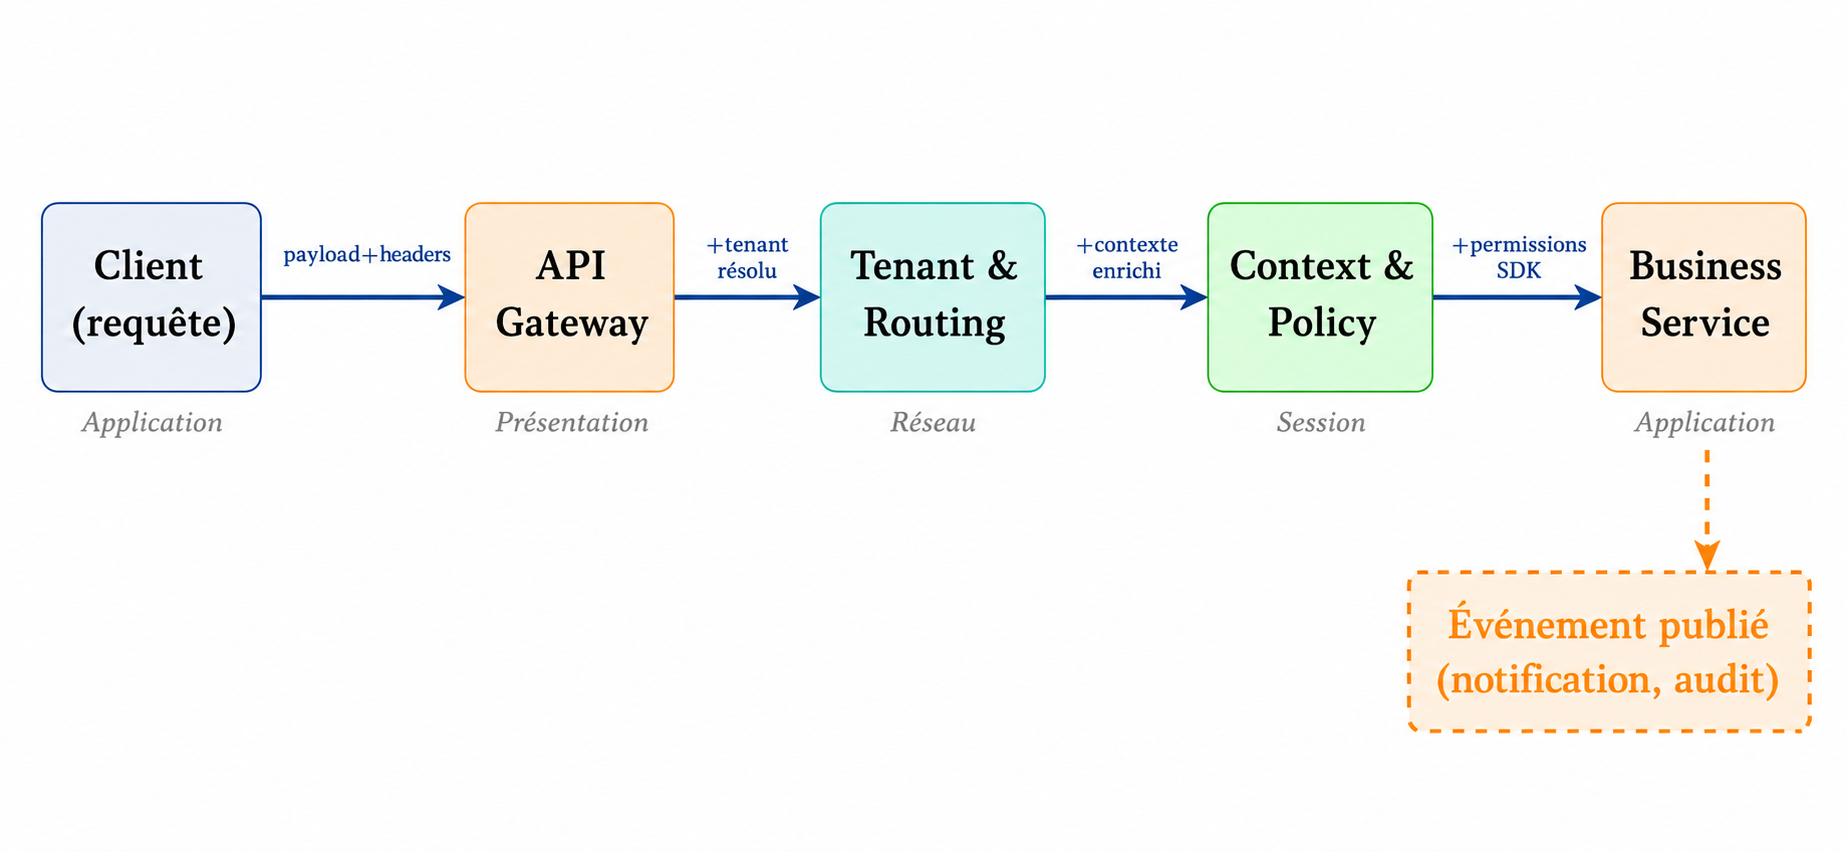
\includegraphics[width=\textwidth]{figures/flux_de_traitement_requete.png}
  \caption{Flux bout-en-bout d'une requête dans BCaaS : Client $\to$ API Gateway $\to$ Tenant \& Routing $\to$ Context \& Policy $\to$ Business Service, avec correspondance OSI descendante/ascendante et publication d'événements (notification, audit).}
  \label{fig:flux}
\end{figure}

\section{La pile protocolaire métier en cinq couches}

De l'analogie découle une décomposition de BCaaS en cinq couches protocolaires, en
correspondance directe avec le modèle OSI (figure~\ref{fig:pile}). Chaque couche n'expose
qu'un service bien défini à la couche supérieure.

\begin{figure}[h]
	\centering
	\begin{tikzpicture}[
		layer/.style={draw=#1, fill=#1!15, minimum width=8cm, minimum height=1cm,
			align=center, font=\small\bfseries, rounded corners=3pt},
		rlabel/.style={font=\footnotesize\itshape, text=gray, text width=3.5cm, align=right}
		]
		% Couches
		\node[layer=orange]  (l5) at (0,5.5) {Couche 5 - Business Capabilities};
		\node[layer=green!60!black] (l4) at (0,4.2) {Couche 4 - Context \& Policy};
		\node[layer=teal]    (l3) at (0,2.9) {Couche 3 - Tenant \& Routing};
		\node[layer=blue]    (l2) at (0,1.6) {Couche 2 - Transport \& Messaging};
		\node[layer=blue!40!black] (l1) at (0,0.3) {Couche 1 - Infrastructure};
		
		% Labels droite (analogie OSI)
		\node[rlabel] at (6.5,5.5) {Application};
		\node[rlabel] at (6.5,4.2) {Session / Présentation};
		\node[rlabel] at (6.5,2.9) {Réseau};
		\node[rlabel] at (6.5,1.6) {Transport};
		\node[rlabel] at (6.5,0.3) {Physique / Liaison};
		
		% Labels gauche (technologies)
		\node[font=\tiny, text=gray, align=left, text width=2.5cm] at (-5.5,5.5)
		{Acteurs, Ressources, Workflows, Audit};
		\node[font=\tiny, text=gray, align=left, text width=2.5cm] at (-5.5,4.2)
		{JWT, RBAC, Politiques, Saga};
		\node[font=\tiny, text=gray, align=left, text width=2.5cm] at (-5.5,2.9)
		{TenantResolver, API Gateway};
		\node[font=\tiny, text=gray, align=left, text width=2.5cm] at (-5.5,1.6)
		{REST, gRPC, Kafka, Redis};
		\node[font=\tiny, text=gray, align=left, text width=2.5cm] at (-5.5,0.3)
		{PostgreSQL, Docker, Prometheus};
		
		% Accolades
		\draw[decorate, decoration={brace,amplitude=6pt}, primary, line width=1pt]
		(4.5,0) -- (4.5,6.2) node[midway, right=10pt, font=\footnotesize, primary]
		{\textbf{Analogie OSI}};
	\end{tikzpicture}
	\caption{Pile protocolaire métier de \bcaas{} et correspondance avec le modèle OSI}
	\label{fig:pile}
\end{figure}

\subsection{Couche 1 --- Infrastructure}
Substrat technique : base de données PostgreSQL avec migrations Liquibase, cache Redis et
bus de messages. Elle correspond aux couches physique et liaison : elle transporte les
données sans en connaître la signification.

\subsection{Couche 2 --- Transport \& Messaging}
Analogue à la couche transport (TCP/UDP). Elle gère le mode d'échange (synchrone via REST,
ou asynchrone via le bus d'événements), les stratégies de retry, les timeouts et
l'idempotence. Le choix \emph{REST $\equiv$ TCP} (fiable, ordonné) ou \emph{événement
$\equiv$ UDP} (rapide, au mieux) est explicite dans la conception.

\subsection{Couche 3 --- Tenant \& Routing}
Analogue à la couche réseau. Le \emph{Tenant Resolver} joue le rôle d'un routeur : à partir
de l'en-tête de la requête (le claim \texttt{tenantId} du JWT), il détermine le contexte
d'exécution et oriente la requête vers le bon service. C'est ici que réside la logique de
découverte et d'isolation.

\subsection{Couche 4 --- Context \& Policy}
Analogue aux couches session et présentation. Cette couche valide le token JWT, décode les
rôles et permissions, applique les politiques de sécurité propres au tenant et détermine le
niveau de service. C'est ici qu'est construit l'« en-tête métier » complet de la requête.

\subsection{Couche 5 --- Business Capabilities}
Couche applicative. Elle contient les services métier génériques (acteurs, métiers,
services, ressources, règles, factures, audit), qui opèrent sur des données configurables
par tenant sans connaissance des couches inférieures.

\section{Le multi-tenant comme réseau virtuel (VLAN)}

\begin{analogie}[Analogie : VLAN $\leftrightarrow$ Tenant]
Dans un réseau, un VLAN isole logiquement plusieurs groupes de machines sur la même
infrastructure physique ; chaque trame porte un \emph{tag} (802.1Q) identifiant son
appartenance. Dans BCaaS, chaque requête porte un \texttt{tenant\_id} qui isole les
données, les règles et les workflows d'un client sur l'infrastructure partagée.
\[
\text{tag VLAN} \;\equiv\; \texttt{tenant\_id}, \qquad
\text{réseau physique} \;\equiv\; \text{infrastructure partagée}.
\]
\end{analogie}

\section{Plan de contrôle et plan de données}

\begin{analogie}[Analogie : SDN $\leftrightarrow$ Administration BCaaS]
Dans les réseaux définis par logiciel (SDN), le \emph{control plane} configure de façon
centralisée les règles de routage, tandis que le \emph{data plane} achemine les paquets.
Dans BCaaS, l'interface d'administration (control plane) configure tenants, règles métier,
catalogues et niveaux de service ; le moteur d'exécution (data plane) traite les
transactions en appliquant ces configurations, et émet les événements d'audit et de
notification.

\[
\underbrace{\text{Admin API}}_{\text{Control plane}}
\;\xrightarrow{\text{configuration}}\;
\underbrace{\text{Moteur de transactions}}_{\text{Data plane}}
\;\xrightarrow{\text{exécution}}\;
\underbrace{\text{Audit, Notifications}}_{\text{Événements}}
\]

\end{analogie}
\section{Routage applicatif et recherche de chemin logique}
\label{sec:routage_applicatif}

\begin{analogie}[Analogie : Table de Routage $\leftrightarrow$ Workflow Engine / Handler Resolver]
Dans les infrastructures réseaux, le routage consiste à déterminer le chemin optimal qu'un paquet doit emprunter à travers des nœuds intermédiaires pour atteindre sa destination, en se basant sur des tables de routage dynamiques (alimentées par OSPF ou BGP). 

Dans la plateforme BCaaS, nous transposons ce mécanisme sous la forme d'un \emph{Handler Resolver} couplé à un moteur de règles. Lorsqu'une \texttt{ServiceRequest} franchit les couches de sécurité, le cœur du système inspecte les métadonnées de la requête (le type de service et l'action demandée). À l'instar d'un routeur effectuant un \emph{longest prefix match} sur une adresse IP, le moteur BCaaS effectue une résolution dynamique pour aiguiller le message vers l'instance de composant métier (\emph{Service Handler}) configurée pour ce tenant spécifique.
\end{analogie}

\section{Contrôle de flux et qualité de service (QoS)}
\label{sec:qos_flux}

\begin{analogie}[Analogie : QoS / Token Bucket $\leftrightarrow$ Rate Limiting et SLA]
La mise en commun des ressources physiques au sein d'une infrastructure partagée expose le système au syndrome du \emph{Noisy Neighbor} (un utilisateur saturant les ressources au détriment des autres). En ingénierie des réseaux, ce problème est résolu par des politiques de Qualité de Service (QoS) et des algorithmes de lissage de trafic comme le \emph{Token Bucket}, qui limitent le débit d'un flux à une bande passante allouée.

Au niveau de BCaaS, cette gestion des congestions est implémentée par un mécanisme de \emph{Rate Limiting} adossé aux contrats de niveau de service (\emph{SLA}) des tenants. Chaque requête entrante est soumise à un compteur glissant (géré en cache haute performance via Redis). Si un tenant dépasse le quota de transactions par seconde (TPS) stipulé par ses règles de configuration, le système applique un contrôle de flux strict en rejetant les requêtes excédentaires avec un code statut HTTP 429 (\emph{Too Many Requests}), préservant ainsi la disponibilité globale du \emph{Business Core}.
\end{analogie}


